\documentclass[11pt]{article}

\usepackage[italian]{babel}
\usepackage[utf8]{inputenc}  
\usepackage[normalem]{ulem}
\usepackage[table,xcdraw]{xcolor}
\usepackage{amsmath}         
\usepackage{amssymb}         
\usepackage{graphicx}        
\usepackage{geometry}        
\usepackage{fancyhdr}            
\usepackage{float} 
\usepackage{tabularx}
\usepackage{multicol}
\usepackage{caption}
\usepackage{tcolorbox} 
% Impostazioni per i margini
\geometry{a4paper, margin=0.76in}

% Grandezza righe tabelle
\renewcommand{\arraystretch}{1.2} % Aumenta l'altezza delle righe

% Intestazioni
\pagestyle{fancy}
\fancyhf{}
\fancyhead[L]{Linguaggi Formali e Compilatori}
\fancyhead[R]{Soluzione Esercizi Tipo - Parte I}
\fancyfoot[C]{\thepage}   
\setlength{\headheight}{14pt}

\begin{document}
%%%%%%%%%%%%%%%%%%%%%%% ESERCIZIO 1 %%%%%%%%%%%%%%%%%%%%%%%
\section*{Esercizio 1}
Se due linguaggi sono regolari allora la loro unione è regolare, 
basta prendere i due DFA che riconoscono i linguaggi e creare un nuovo
stato iniziale che si collega agli stati iniziali dei due DFA tramite
una $\epsilon$-transizione quindi la risposta è \textbf{VERO}.
%%% Nota inizia qui %%%
\begin{tcolorbox}[colframe=orange!70!black, colback=orange!10!white, title=\textbf{\textit{Nota \sout{inutile ai fini dell'esercizio}:}}]
Se prendessimo ad esempio:
\begin{itemize}
  \item ${\cal L}_1 = \{w \in \{a,b\}^*|\;w\;ha\;una\;lunghezza\;pari\}$  
  \item ${\cal L}_2 = \{w \in \{a,b\}^*|\;w\;termina\;con\;a\}$  
\end{itemize}
\begin{multicols}{2}
  \begin{figure}[H]
  \centering
    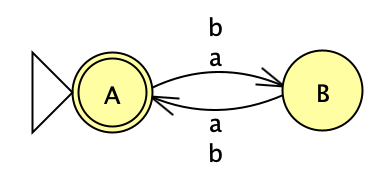
\includegraphics[height=2.5cm]{img/01Pari.png}
    \label{fig:01-DFA-pari}
    \caption*{DFA per ${\cal L}_1$}
  \end{figure}
  \begin{figure}[H]
  \centering
    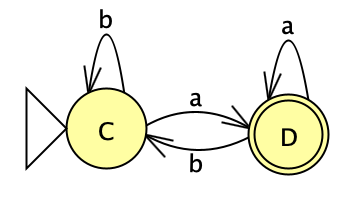
\includegraphics[height=2.5cm]{img/01FinisceConA.png}
    \label{fig:01-DFA-finisce-con-a}
    \caption*{DFA per ${\cal L}_2$}
  \end{figure}
\end{multicols}
L'unione di  ${\cal L}_1$ con  ${\cal L}_2$ sta a significare che la 
parola su $\{a, b\}$ deve essere pari oppure finire con la lettera $a$.
Per costruire l'automa che verifichi l'unione potremo leggere la parola
contemporaneamente in entrambi i DFA e se al termine della parola mi 
trovo in uno stato finale di uno dei due DFA allora la parola appartiene
all'unione.

Possiamo costruire il DFA finale quindi facendo il prodotto cartesiano
degli stati, quello iniziale sarà $AC$ mentre quelli finali saranno 
$AC$, $AD$ e $BD$ ottenendo il seguente DFA, confermando che l'unione 
è regolare.
\begin{figure}[H]
  \centering
  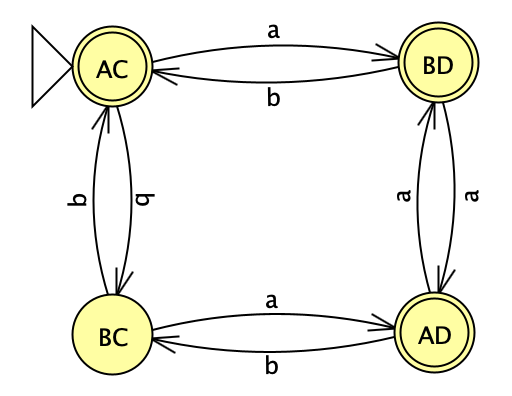
\includegraphics[height=4.3cm]{img/01Unione.png}
  \label{fig:01-DFA-unione}
\end{figure}
\noindent Andando ad 'occhio' si poteva comunque costruire un DFA 
che riconosceva ${\cal L}_1 \cup {\cal L}_2$:
\begin{figure}[H]
  \centering
  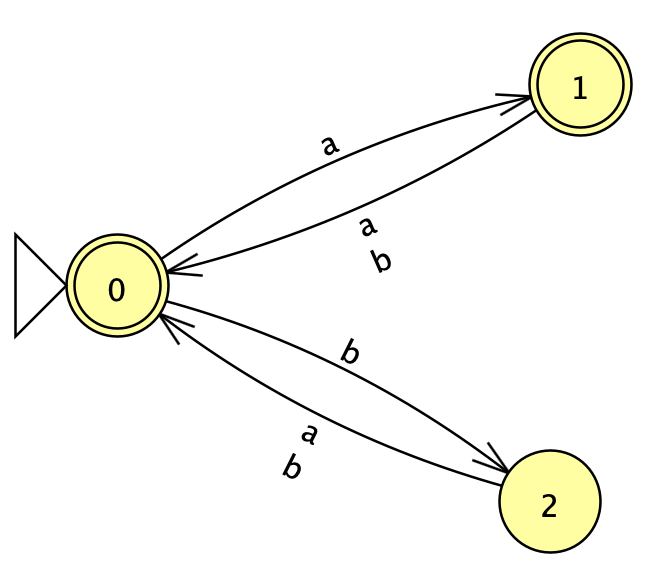
\includegraphics[height=4.3cm]{img/01Unione-1.png}
  \label{fig:01-DFA-unione-1}
\end{figure} 
\end{tcolorbox}
%%% Nota finisce qui %%%
%%%%%%%%%%%%%%%%%%%%%%% ESERCIZIO 2 %%%%%%%%%%%%%%%%%%%%%%%
\section*{Esercizio 2}
Sulle slide o dispensa studenti.
\newpage
%%%%%%%%%%%%%%%%%%%%%%% ESERCIZIO 3 %%%%%%%%%%%%%%%%%%%%%%%
\section*{Esercizio 3}
Per la costruzione di un DFA da un NFA partiamo dallo
stato iniziale $A$ e calcoliamo la sua $\epsilon$-chiusura:
$$closure(A) = \{A\;,B,\;C,\;E\} = T_0$$
Controllando le transazioni da $T_0$:
\begin{itemize}
  \item a-transizione: $closure(D,\;E) = \{D,\;E\} = T_1$
  \item b-transizione: $closure(A,\;E) = \{A\;,B,\;C,\;E\} = T_0$
\end{itemize}
$T_1$:
\begin{itemize}
  \item a-transizione: $closure(E) = \{E\} = T_2$
  \item b-transizione: $closure(A,\;B) = \{A\;,B,\;C,\;E\} = T_0$
\end{itemize}
$T_2$:
\begin{itemize}
  \item a-transizione: $closure(E) = \{E\} = T_2$
  \item b-transizione: $closure(A) = \{A\;,B,\;C,\;E\} = T_0$
\end{itemize}
La funzione di transazione del DFA sarà:
\begin{table}[H]
  \centering
  \begin{tabularx}{\textwidth}{|>{\centering\arraybackslash}X|>{\centering\arraybackslash}X|>{\centering\arraybackslash}X|}
  \hline
  & \textbf{a} & \textbf{b}  \\
  \hline
  $T_0$ & $T_1$ & $T_0$\\
  \hline
  $T_1$ & $T_2$ & $T_0$ \\
  \hline
  $T_2$ & $T_2$ & $T_0$ \\
  \hline
  \end{tabularx}
  \label{tab:03-parsing-table}
\end{table}
\noindent Quindi se $Q$ è lo stato iniziale del DFA allora: $Q[ab] = T_0 = {A, B, C, E}$
\begin{figure}[H]
  \centering
  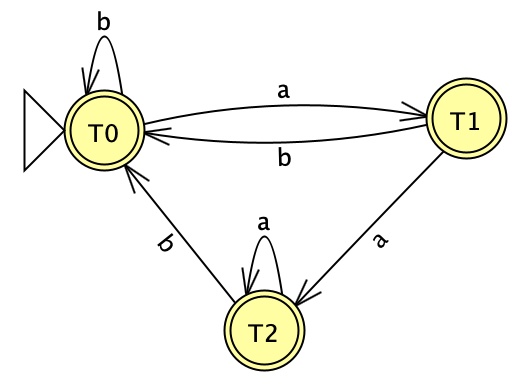
\includegraphics[height=4cm]{img/03DFA.png}
  \label{fig:03-DFA}
\end{figure} 
%%%%%%%%%%%%%%%%%%%%%%% ESERCIZIO 4 %%%%%%%%%%%%%%%%%%%%%%%
\section*{Esercizio 4}
\cal D ha una funzione di transizione parziale. Per renderla totale, aggiungiamo uno stato 'sink' che assorbe tutte le transizioni non definite:

\begin{multicols}{2}
  \begin{figure}[H]
    \centering
    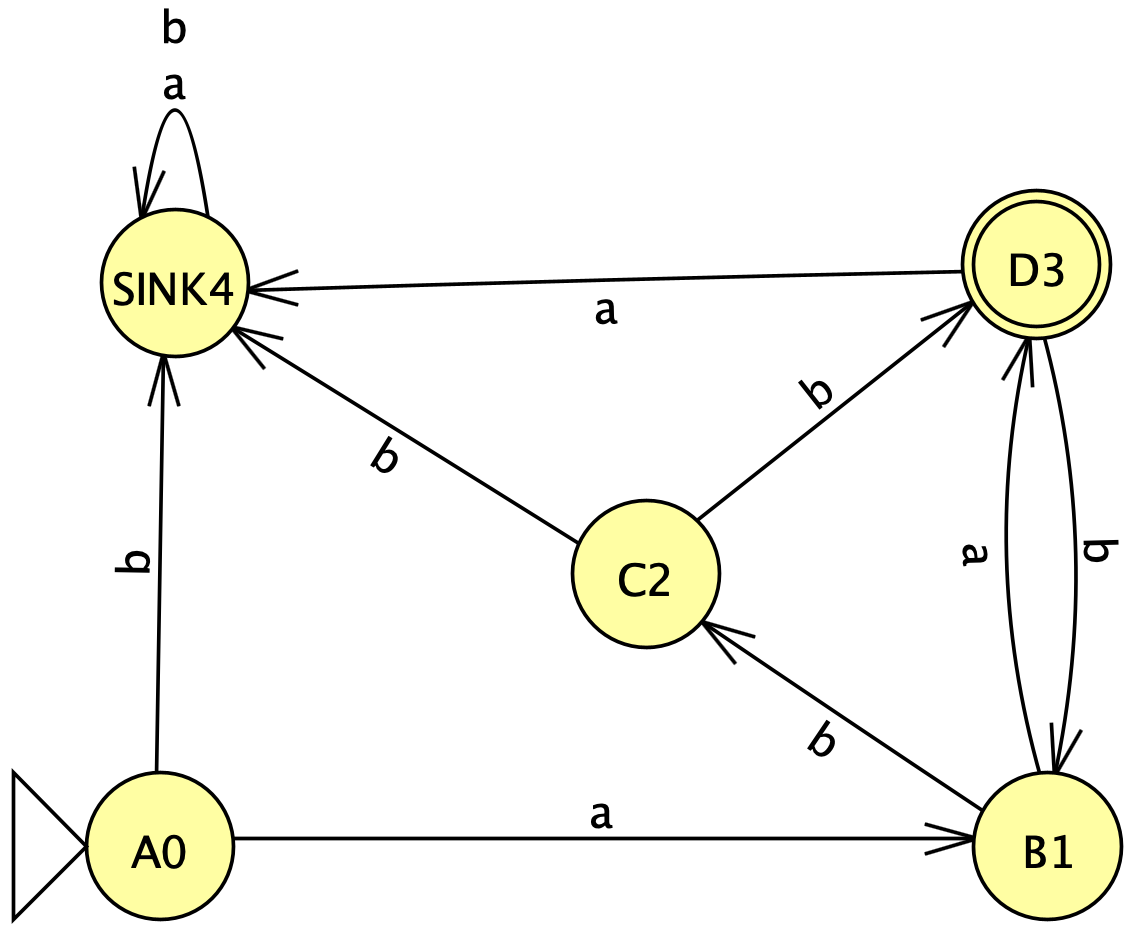
\includegraphics[height=4cm]{img/04DFAsink.png}
    \label{fig:04-DFA-sink}
  \end{figure}
  
  \begin{table}[H]
    \centering
    \begin{tabularx}{\linewidth}{|>{\centering\arraybackslash}X|>{\centering\arraybackslash}X|>{\centering\arraybackslash}X|}
    \hline
    & \textbf{a} & \textbf{b}  \\
    \hline
    $A$ & $B$ & $Sink$ \\
    \hline
    $B$ & $D$ & $C$ \\
    \hline
    $C$ & $D$ & $Sink$ \\
    \hline
    $D$ & $Sink$ & $B$ \\
    \hline
    $Sink$ & $Sink$ & $Sink$ \\
    \hline
    \end{tabularx}
    \label{tab:04-funzione-transazione}
    \caption*{\small Funzione di Transizione}
  \end{table}
\end{multicols}

\noindent Per minimizzare l'automa, analizziamo gli stati di equivalenza usando il \textit{partition refinment}:

\begin{table}[H]
  \small
  \centering
  \begin{tabularx}{\linewidth}{l l l l l l}
  0-equivalenti & $\{A,\;B,\;C,\;Sink\}$ & $\{D\}$ & & & \\
  1-equivalenti & $\{A,\;Sink\}$ & $\{B,\;C\}$ & $\{D\}$ & & \\
  2-equivalenti & $\{A\}$ & $\{Sink\}$ & $\{B\}$ & $\{C\}$ & $\{D\}$ \\
  \end{tabularx}
  \label{tab:04-partition-refinment}
\end{table}

\begin{tcolorbox}[colframe=orange!70!black, colback=orange!10!white, title=\textbf{\textit{Spiegazione}}]
\begin{itemize}
    \item \textbf{Stati 0-equivalenti}: si distinguono gli stati finali e non finali
    \item \textbf{Stati 1-equivalenti}: 
    \begin{itemize}
      \item $\{A, Sink\}$ transitano entrambi verso lo stesso insieme $\{A,\;B,\;C,\;Sink\}$ sia con \textit{a-transazione} che con \textit{b-transazione}
      \item $\{B, C\}$ transitano entrambi verso lo stesso insieme $\{D\}$ con \textit{a-transazione} e in $\{A,\;B,\;C,\;Sink\}$ con \textit{b-transazione}.
    \end{itemize}
    \item \textbf{Stati 2-equivalenti}:
    \begin{itemize}
      \item $A$ e $Sink$ vanno divisi perché la \textit{a-transazione} li porta a due insiemi diversi (A va a $\{B, C\}$ mentre Sink va a $\{A, Sink\}$)
      \item in modo analogo anche $B$ e $C$ vanno separati perché la \textit{b-transazione} li porta a due insiemi diversi
    \end{itemize}
\end{itemize}
\end{tcolorbox}
\noindent 
Il DFA è già minimo poiché nessun raggruppamento è possibile. \\
Quindi lo stato a cui corrisponde $P[abab]$ è $B$.
%%%%%%%%%%%%%%%%%%%%%%% ESERCIZIO 5 %%%%%%%%%%%%%%%%%%%%%%%
\section*{Esercizio 5}
Iniziamo calcolando i $first$ e i $follow$.
\begin{multicols}{2}
\noindent\textbf{First:}
\begin{itemize}
  \item B può derivare $\epsilon$. Pertanto, $first(B) = \{\epsilon\}$
  \item A può derivare $BcBaA$ quindi aggiungiamo i $first(B)$ ai $first(A)$, $first(B)$ contiene $\epsilon$
  quindi consideriamo $first(cBaA)$ e aggiungiamo $c$ ai $first(A)$,
  A può anche derivare $\epsilon$ quindi aggiungiamola ai $first(A)$
  \item S può derivare $AaB$ quindi aggiungiamo i $first(A)$ ai $first(S)$,
  essendoci $\epsilon$ nei $first(A)$ allora dobbiamo aggiungere $first(aB)$ ai $first(S)$, infine S può derivare $b$ che sarà da aggiungere ai suoi $first$ 
\end{itemize}
\begin{table}[H]  
  \centering
  \begin{tabularx}{\linewidth}{|>{\centering\arraybackslash}X|>{\centering\arraybackslash}X|>{\centering\arraybackslash}X|}
    \hline
    & first & follow  \\
    \hline
    $S$ & b a c & \$ \\
    \hline
    $A$ & $\epsilon$ c & a \\
    \hline
    $B$ & $\epsilon$ & c a \$ \\
    \hline
  \end{tabularx}
  \label{tab:05-first-follow}
\end{table}
\textbf{Follow:} 
\begin{itemize}
  \item $follow(S)$: S è lo start symbol, quindi $follow(S) = \{\$\}$, S non compare in nessun body quindi ci possiamo fermare
  \item $follow(A)$: nella produzione $S \to AaB$, A è seguito da 'aB', quindi $first(aB) = \{a\}$ è in $follow(A)$
  \item $follow(B)$:
  \begin{itemize}
    \item nella produzione $S \to AaB$, B è l'ultimo simbolo della produzione dobbiamo aggiungere i $follow(S)$ ai $follow(B)$
    \item nella produzione $A \to BcBaA$, B è seguito da 'cBaA', $first(cBaA) = \{c\}$ è in $follow(B)$
  \end{itemize} 
\end{itemize}
\end{multicols}
\newpage
Le regole per popolare la tabella di parsing LL(1) sono:
\begin{itemize}
  \item per ogni produzione $A \to \alpha$ nella grammatica:
  \begin{itemize}
     \item per ogni terminale 'b' in $first(\alpha)$ (escludendo $\epsilon$) bisogna aggiungere $A \to \alpha$ alla voce della tabella $M[A, b]$.
     \item se $\epsilon$ è in $first(\alpha)$ allora per ogni terminale 'x' in $follow(A)$ bisogna aggiungere $A \to \alpha$ alla voce della tabella $M[A, x]$.
  \end{itemize}
  \item imposta tutte le voci vuote nella tabella a 'errore'
\end{itemize}
La tabella di parsing $LL(1)$ è la seguente e la risposta è evidenziata:
\begin{table}[H]
  \centering
  \begin{tabularx}{\linewidth}{|X|X|X|X|X|}
    \hline
    & \textbf{a} & \textbf{b} & \textbf{c} & \textbf{\$} \\
    \hline
    $S$ & $S\rightarrow AaB$ & $S\rightarrow b$ & $S\rightarrow AaB$ & \\
    \hline
    $A$ & $A\rightarrow \epsilon$ & & $A\rightarrow BcBaA$& \\
    \hline
    \rowcolor{yellow}
    $B$ & $B\rightarrow \epsilon$ & & $B\rightarrow \epsilon$ & $B\rightarrow \epsilon$ \\
    \hline
    \end{tabularx}
  \label{tab:05-tabella-parsing}
\end{table}
\section*{Esercizio 6}
$${\cal L} = \{ww | w \in {\cal L}((a|b)^*)\}$$
Questo linguaggio rappresenta l'insieme delle stringhe formate da due
copie consecutive di una parola del linguaggio denotato da $(a|b)^*$.
\\Per dimostrare che non è regolare utilizzando il pumping lemma:
\begin{enumerate}
  \item supponiamo che $\cal L$ sia regolare
  \item prendiamo una \textit{pumping constant} p arbitraria
  \item scegliamo una parola opportuna $z=a^p\,b^p\,a^p\,b^p$
  \item guardiamo a tutte le possibili decomposizioni di $z$ in $uvw$ con:
  \begin{enumerate}
    \item $|uv| \le p$
    \item $|v| \ge 1$
  \end{enumerate}
  Quindi abbiamo che $u=a^\alpha$, $v=a^\beta$ e $w=a^{p -\alpha - \beta }\,b^p\,a^p\,b^p$
  \item scelgo una $i$ opportuna tale che $uv^iw \not \in \cal L$
  $$a^\alpha\,a^{i\cdot\beta}\,a^{p-\alpha -\beta}\,b^p\,a^p\,b^p = a^{p + \beta (i -1)}\,b^p\,a^p\,b^p$$
  Sapendo che $\beta \ne 0$ perché $|v| \ge 1$ ci basta scegliere $i \ne 1$, quindi scegliamo 2 e otteniamo 
  $$a^{p + \beta}\,b^p\,a^p\,b^p \not \in \cal L$$ 
\end{enumerate}
Andando così in contraddizione con l'enunciato del pumping lemma, quindi $\cal L$ non è regolare.
\newpage
\section*{Esercizio 7}
Un metodo per risolvere questo esercizio sarebbe quello di fare la \textit{costruzione
di Thompson} per ottenere un NFA, dopo di che fare il \textit{subset construction} per tradurlo in un DFA ed infine il \textit{partition refinment} per minimizzarlo.
Solo che all'esame, non si ha tutto questo tempo, quindi possiamo analizzare la regex:
\begin{itemize}
  \item $b^*$ denota o la parola vuota oppure una serie arbitraria di b
  \item $b^*\,a\,(\epsilon\,|\,a\,|\,b)^*$ denota una serie arbitraria di $b$ (anche zero) seguita da una a seguita da $(a | b)^*$
\end{itemize}
Si riescie a notare che possiamo formare qualsiasi parola su $\{a, b\}$, quindi l'automa caratteristico può essere il seguente:
\begin{figure}[H]
  \centering
  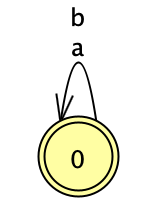
\includegraphics[height=2.5cm]{img/07DFA.png}
  \label{fig:07-DFA}
\end{figure}
\noindent Che è già minimo. Quindi la risposta è che $\cal D$ ha uno stato che è anche finale.

\section*{Esercizi 8, 9 e 10}
Guardare \textbf{5.4 Proprietà di chiusura nei linguaggi regolari} della dispensa studenti.
\end{document}
